\documentclass[../../main/main.tex]{subfiles}
\graphicspath{{./figures/}}

\dominitoc
\faketableofcontents

\renewcommand{\mtcSfont}{\small\bfseries}
\renewcommand{\mtcSSfont}{\footnotesize}
\mtcsettitle{minitoc}{}
\mtcsetrules{*}{off}

\makeatletter
\renewcommand{\@chapapp}{Physique quantique -- chapitre}
\makeatother

% \toggletrue{student}
% \toggletrue{corrige}
% \renewcommand{\mycol}{black}
% \renewcommand{\mycol}{gray}

\hfuzz=5.002pt

\begin{document}
\setcounter{chapter}{0}
\chapter{Introduction à la physique quantique}
\label{ch:mecaq}

\settype{book}
\settype{prof}
\settype{stud}

\epigraph{\openquote\textit{%
		Those who are not shocked when they first come across quantum theory cannot possibly have understood it.
	}%
	\closequote}{Niels \textsc{Bohr}, 1952, Copenhague}

\vspace*{\fill}

\begin{tcn}(appl)<ctc>"somm"'t'{Sommaire}
	\let\item\olditem
	\vspace{-15pt}
	\minitoc
	\vspace{-25pt}
\end{tcn}

\begin{tcn}[sidebyside, fontupper=\small, fontlower=\small](appl)<ctb>"how"'t'{Capacités exigibles}
	\begin{itemize}[label=\rcheck]
		\item Décrire un exemple d'expérience mettant en évidence la nécessité de la
		      notion de photon.

		\item Décrire un exemple d'expérience mettant en évidence le comportement
		      ondulatoire de la matière.

		\item Évaluer des ordres de grandeurs typiques intervenant dans des
		      phénomènes quantiques.

	\end{itemize}
	\tcblower
	\begin{itemize}[label=\rcheck]
		\item Interpréter une expérience d’interférences (matière ou lumière)
		      «~particule par particule~» en termes probabilistes.

		\item Inégalité de \textsc{Heisenberg} spatiale~: établir par analogie avec la
		      diffraction des ondes lumineuses, l’inégalité en ordre de grandeur~:
		      $\Delta{p}\Delta{x} \geq \h$.

		\item Modèle de \textsc{Bohr}~: exploiter l’hypothèse de quantification du
		      moment cinétique orbital pour obtenir l’expression des niveaux d’énergie
		      électronique de l’atome d’hydrogène.

	\end{itemize}
\end{tcn}

% \vspace{-15pt}

\vspace*{\fill}

\newpage

\vspace*{\fill}
% {%
% \begin{boxes}
\begin{tcn}[sidebyside, fontupper=\small, fontlower=\small](appl)<ctb>"chek"'t'{L'essentiel}
	\begin{tcn}(defi)<ctc>'t'{Définitions}
		\tcblistof[\paragraph*]{defi}{\hspace*{4.8pt}}
	\end{tcn}
	% \begin{tcn}(rapp)<ctc>'t'{Rappels}
	% 	\tcblistof[\paragraph*]{rapp}{\hspace*{4.8pt}}
	% \end{tcn}
	\begin{tcn}(prop)<ctc>'t'{Propriétés}
		\tcblistof[\paragraph*]{prop}{\hspace*{4.8pt}}
		\tcblistof[\paragraph*]{loi}{\hspace*{4.8pt}}
		% \tcblistof[\paragraph*]{theo}{\hspace*{4.8pt}}
	\end{tcn}
	% \begin{tcn}(coro)<ctc>'t'{Corollaires}
	%   \tcblistof[\paragraph*]{coro}{\hspace*{4.8pt}}
	% \end{tcn}
	% \begin{tcn}(demo)<ctc>'t'{Démonstrations}
	% 	\tcblistof[\paragraph*]{demo}{\hspace*{4.8pt}}
	% 	\tcblistof[\paragraph*]{prev}{\hspace*{4.8pt}}
	% \end{tcn}
	% \begin{tcn}(inte)<ctc>'t'{Interprétations}
	% 	\tcblistof[\paragraph*]{inte}{\hspace*{4.8pt}}
	% \end{tcn}
	% \begin{tcn}(impl)<ctc>'t'{Implications}
	% 	\tcblistof[\paragraph*]{impl}{\hspace*{4.8pt}}
	% \end{tcn}
	% \begin{tcn}(tool)<ctc>'t'{Outils}
	% 	\tcblistof[\paragraph*]{tool}{\hspace*{4.8pt}}
	% \end{tcn}
	% \begin{tcn}(nota)<ctc>'t'{Notations}
	%   \tcblistof[\paragraph*]{nota}{\hspace*{4.8pt}}
	% \end{tcn}
	% \begin{tcn}(appl)<ctc>'t'{Applications}
	% 	\tcblistof[\paragraph*]{appl}{\hspace*{4.8pt}}
	% \end{tcn}
	% \begin{tcn}(rema)<ctc>'t'{Remarques}
	%   \tcblistof[\paragraph*]{rema}{\hspace*{4.8pt}}
	% \end{tcn}
	% \begin{tcn}(exem)<ctc>'t'{Exemples}
	% 	\tcblistof[\paragraph*]{exem}{\hspace*{4.8pt}}
	% \end{tcn}
	% \begin{tcn}*(ror)<ctc>"hart"'t'{Points importants}
	%   \tcblistof[\paragraph*]{ror}{\hspace*{4.8pt}}
	% \end{tcn}
	% \begin{tcn}(impo)<ctc>'t'{Erreurs communes}
	%   \tcblistof[\paragraph*]{impo}{\hspace*{4.8pt}}
	% \end{tcn}
	\tcblower
	% \begin{tcn}(defi)<ctc>'t'{Définitions}
	%   \tcblistof[\paragraph*]{defi}{\hspace*{4.8pt}}
	% \end{tcn}
	% \begin{tcn}(rapp)<ctc>'t'{Rappels}
	%   \tcblistof[\paragraph*]{rapp}{\hspace*{4.8pt}}
	% \end{tcn}
	% \begin{tcn}(prop)<ctc>'t'{Propriétés}
	%   \tcblistof[\paragraph*]{prop}{\hspace*{4.8pt}}
	%   \tcblistof[\paragraph*]{loi}{\hspace*{4.8pt}}
	%   \tcblistof[\paragraph*]{theo}{\hspace*{4.8pt}}
	% \end{tcn}
	% \begin{tcn}(coro)<ctc>'t'{Corollaires}
	%   \tcblistof[\paragraph*]{coro}{\hspace*{4.8pt}}
	% \end{tcn}
	% \begin{tcn}(demo)<ctc>'t'{Démonstrations}
	% 	\tcblistof[\paragraph*]{demo}{\hspace*{4.8pt}}
	% 	\tcblistof[\paragraph*]{prev}{\hspace*{4.8pt}}
	% \end{tcn}
	% \begin{tcn}(inte)<ctc>'t'{Interprétations}
	% 	\tcblistof[\paragraph*]{inte}{\hspace*{4.8pt}}
	% \end{tcn}
	\begin{tcn}(impl)<ctc>'t'{Implications}
		\tcblistof[\paragraph*]{impl}{\hspace*{4.8pt}}
	\end{tcn}
	% \begin{tcn}(tool)<ctc>'t'{Outils}
	%   \tcblistof[\paragraph*]{tool}{\hspace*{4.8pt}}
	% \end{tcn}
	% \begin{tcn}(nota)<ctc>'t'{Notations}
	%   \tcblistof[\paragraph*]{nota}{\hspace*{4.8pt}}
	% \end{tcn}
	% \begin{tcn}(odgr)<ctc>'t'{Ordres de grandeur}
	% 	\tcblistof[\paragraph*]{odgr}{\hspace*{4.8pt}}
	% \end{tcn}
	% \begin{tcn}(appl)<ctc>'t'{Applications}
	% 	\tcblistof[\paragraph*]{appl}{\hspace*{4.8pt}}
	% \end{tcn}
	% \begin{tcn}(rema)<ctc>'t'{Remarques}
	%   \tcblistof[\paragraph*]{rema}{\hspace*{4.8pt}}
	% \end{tcn}
	\begin{tcn}(exem)<ctc>'t'{Exemples}
		\tcblistof[\paragraph*]{exem}{\hspace*{4.8pt}}
	\end{tcn}
	\begin{tcn}*(ror)<ctc>"hart"'t'{Points importants}
		\tcblistof[\paragraph*]{ror}{\hspace*{4.8pt}}
	\end{tcn}
	\begin{tcn}(impo)<ctc>'t'{Erreurs communes}
		\tcblistof[\paragraph*]{impo}{\hspace*{4.8pt}}
	\end{tcn}
\end{tcn}
% \end{boxes}
% }%

\vspace*{\fill}
\newpage

\section{Un peu d'histoire}
\label{sec:mqhistoire}
Dans notre vie quotidienne, nous interagissons avec des systèmes à une échelle
macroscopique, qu'on modélise assez correctement en physique par un assemblage
de systèmes à l'échelle mésoscopique. L'idée de trouver une brique élémentaire à
ce qui compose notre monde, qui nous donnerait des clés pour le comprendre en le
prédire en totalité, est naturellement une idée ancienne. Le concept premier
d'«~atome~», du grec \textit{atomos}, «~insécable~», pensé par
\textsc{Démocrite} et \textsc{Épicure}, traduisait cette brique fondamentale
hypothétique. Cependant, l'accès expérimental à cette potentielle réalité
physique est resté difficile pendant de nombreux siècles.
% TODO: Citation on connaîtrait tout le monde avec les CI~: Laplace.
\bigbreak
En attendant, la majeure partie du monde physico-chimique tel qu'on le concevait
a été étudié et décrit~: la mécanique des solides et la mécanique des fluides,
la thermodynamique et la thermochimie, les ondes sonores et l'optique
géométrique… mais les questions sur la nature profonde de certains phénomènes
restent ouvertes, et de vifs débats enflamment les plus grands esprits.
\bigbreak
Au début du \textsc{xx}\ieme\ siècle, la lumière échappe à cette compréhension
profonde. Les outils existant sont ceux de la mécanique de \textsc{Newton} (fin
du \textsc{xvii}\ieme\ siècle) et l'électromagnétisme de \textsc{Maxwell}
(milieu et fin du \textsc{xix}\ieme\ siècle)~: c'est la physique
\textbf{classique}, description du monde alors très robuste et complètement
déterministe, donnant une raison infiniment claire à toute observation du monde
réel. Cependant, quelques expériences les mettent en défaut~:
\bigbreak
\noindent
\begin{minipage}[c]{.60\linewidth}
	\begin{itemize}
		\item[b]{L'effet photoélectrique}: exposer une plaque métallique exposée à de
		la lumière permet d'en arracher des électrons. Cependant, et ce \textbf{peu
			importe l'intensité du faisceau}, aucun électron n'est arraché si la lumière
		en question est au-dessus d'une certaine longueur d'onde (couleur)~:
		l'éjection \textbf{n'apparaît qu'en-dessous d'une longueur d'onde seuil}
		$\lambda_0$, ce que la physique classique n'explique alors pas encore.
		\bigbreak
		Une proposition de résolution proposée par \textsc{Einstein} est le modèle
		du photon (voir plus loin), \textbf{quantifiant l'énergie} en «~grains~»,
		avec $\Ec$ \textbf{proportionnelle à leur fréquence}, et en supposant qu'un
		électron ne peut absorber \textit{qu'un photon à la fois}. Ainsi, augmenter
		l'intensité du faisceau ne fait qu'augmenter le nombre, mais pas l'énergie
		individuelle.
	\end{itemize}
\end{minipage}
\hfill
\noindent
\begin{minipage}[c]{.35\linewidth}
	\begin{center}
		\sswitch{
			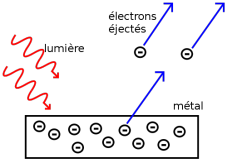
\includegraphics[scale=1, draft=true]{photelec}
		}{
			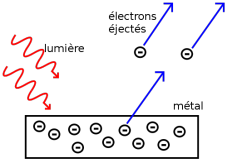
\includegraphics[scale=1]{photelec}
		}
		\captionof{figure}{Éjection des électrons d'un métal sous l'effet d'un
			faisceau lumineux.}
		\label{fig:photelec}
	\end{center}
\end{minipage}
\begin{itemize}
	\item[b]{Raies atomiques}: en excitant un gaz d'un élément unique (comme
	l'hydrogène ou le néon) avec une tension électrique, le milieu dégage de la
	lumière. En la décomposant par un prisme, on obtient alors des raies très
	définies, à l'opposé des spectres continus qu'on observe généralement comme
	celui du soleil par exemple. Cette précision de longueur d'onde émise échappe
	à la physique classique.
	\begin{center}
		\pgfspectra[element=H,
		axis, axis color=white, axis font color=black,
		axis font=\fontsize{10}{12}\selectfont,
		axis ticks=4, axis unit precision=2,
		axis label text={Longueur d'onde [$\si{nm}$]},
		back=white,
		label, label position=north west,
		label before text=Spectre d'émission de~,
		label after text=\ :]
		\captionof{figure}{Spectre \textit{discret} d'émission des raies de
			l'hydrogène.}
		\label{fig:lamp_spec}
	\end{center}
	% \begin{figure}[h!]
	% 	\centering
	% 	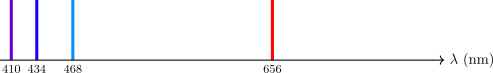
\includegraphics[scale=1]{raiesH-white}
	% 	\caption{Spectre \textit{discret} des raies de l'hydrogène.}
	% 	\label{fig:raiesH}
	% \end{figure}
\end{itemize}

La résolution de ces incompréhensions va mener à la naissance de la mécanique
\textbf{quantique}, issu du latin \textit{quanta}, qui permet une
description des phénomènes physiques non pas comme un ensemble de phénomènes
continus, mais comme un ensemble de phénomènes \textbf{quantifiés}, notamment
\textit{via} des états d'énergie discrets et définis. Par exemple, c'est comme
si on pouvait aller à 50 \textbf{ou} \SI{70}{km.h^{-1}} en voiture, mais pas à
une valeur intermédiaire.
\bigbreak
Cette nouvelle approche du monde va bouleverser la façon de comprendre certains
phénomènes, et est à l'origine d'innombrables applications~: le laser, l'énergie
nucléaire, l'IRM, les semi-conducteurs et donc de toute l'électronique, mais
aussi toute la matière plus généralement et donc les interactions chimiques.

\section{Comportements ondulatoires}
\label{sec:mqonde}
\subsection{Diffraction}
\label{ssec:ondediff}
Une goutte d'eau seule ne fait pas une marrée~: c'est la collection d'objets
tangibles qui se meuvent de manière cohérente qui créé les vagues. On étudie
alors la vague comme un ensemble mais dont on comprend l'origine individuelle.
Une onde présente des propriétés particulières, dont une dont on a déjà parlé au
début de l'année~: la \textbf{diffraction}.
\begin{tcb*}(defi){Diffraction}
	Lorsqu'une onde progressive rencontre un obstacle donc les dimensions sont de
	l'ordre de la longueur d'onde, la partie de l'onde qui la passe subit un
	\textbf{étalement circulaire}, qu'on appelle \textbf{diffraction}.
\end{tcb*}

\noindent
\begin{minipage}[t]{.5\linewidth}
	Une onde plane de longueur d'onde $\lambda$ arrivant sur une fente de taille
	$a \lesssim \lambda$ est diffractée \textit{majoritairement} dans un cône, de
	demi-angle d'ouverture
	\[
		\boxed{\sin{\th} = \frac{\lambda}{a}}
	\]
	soit, pour des petits angles \textbf{en radians},
	\[
		\boxed{\th \Sim_{\th \ll 1} \frac{\lambda}{a}}
	\]
\end{minipage}
\hfill
\begin{minipage}[t]{.45\linewidth}
	~
	\vspace*{-10pt}
	\begin{center}
		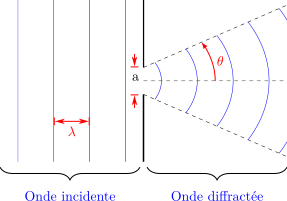
\includegraphics[width=.7\linewidth]{diff1d}
		\captionof{figure}{Diffraction par une fente. Les traits bleus représentent
			les maxima de l'onde.}
		\label{fig:diff1d}
	\end{center}
\end{minipage}

Ce comportement décrit très bien les ondes de matière comme les ondes sonores ou
les vagues arrivant dans un port, mais correspond également à ce que subit la
lumière en passant dans une fente~:
\begin{figure}[h]
	\centering
	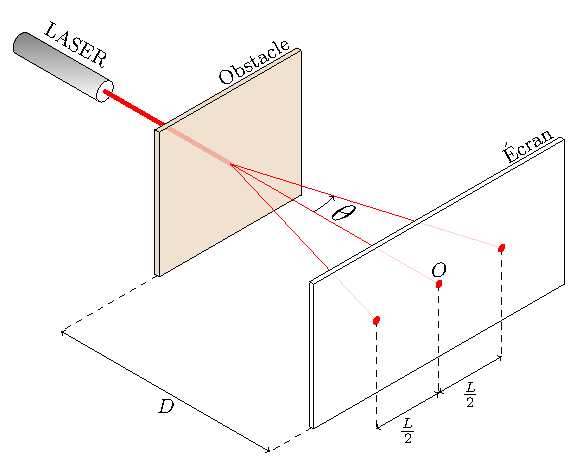
\includegraphics[width=.5\linewidth]{diffraction}
	\caption{Diffraction d'un faisceau laser par une fente fine.}
	\label{fig:diff_las}
\end{figure}

% \begin{tcb*}(appl)<lftt>'l'{Application}
% 	Avec un laser de longueur d'onde $\lambda = \SI{630}{nm}$ et une fente de
% 	largeur $a = \SI{0.1}{mm}$, on observe sur l'écran placé à $D = \SI{5.0}{m}$
% 	une suite de taches de diffraction dont la plus large (au centre) est de
% 	largeur $L$. Calculer cette largeur.
% 	\tcblower
% 	On a $\sin{\th} = \frac{\lambda}{a}$. Or, dans le triangle rectangle formé
% 	par le demi-cône entre la fente et l'écran, on a $\sin{\th} =
% 		\frac{L/2}{D}$~; ainsi
% 	\begin{gather*}
% 		\frac{L}{2D} = \frac{\lambda}{a} \Lra \boxed{L = 2D \frac{\lambda}{a}}
% 		\\
% 		A.N.~: \xul{L = \SI{6.3}{cm}}
% 		\qav
% 		\begin{array}{ll}
% 			D       & = \SI{5.0}{m}
% 			\\
% 			\lambda & = \SI{630e-9}{m}
% 			\\
% 			a       & = \SI{0.1e-3}{m}
% 		\end{array}
% 	\end{gather*}
% \end{tcb*}

\subsection{Interférences}
\label{ssec:ondeint}
Une autre particularité des ondes est le phénomènes d'interférences~:
\begin{tcb*}(defi){Interférence}
	Deux ondes de même nature se rencontrant en un point $\Mr$ se superposent en
	\textbf{sommant leurs signaux}.
\end{tcb*}
Nous avons également décrit ce phénomène plus tôt dans l'année, par l'expérience
des \textbf{fentes d'\textsc{Young}}.
\bigbreak
\noindent
\begin{minipage}{0.45\linewidth}
	La zone de l'espace où les faisceaux se superposent est appelé \textbf{champ
		d'interférences}. Sur un écran, on observe alors la figure ci-contre, avec
	des variations d'intensité lumineuse~:
	\begin{itemize}
		\item au milieu des zones claires (\textbf{maximum} local d'intensité)
		      on a des \textbf{interférences constructives}~;
		\item au milieu des zones sombres (\textbf{minimum} local d'intensité)
		      on a des \textbf{interférences destructives}.
	\end{itemize}
\end{minipage}
\hfill
\begin{minipage}{0.50\linewidth}
	\begin{center}
		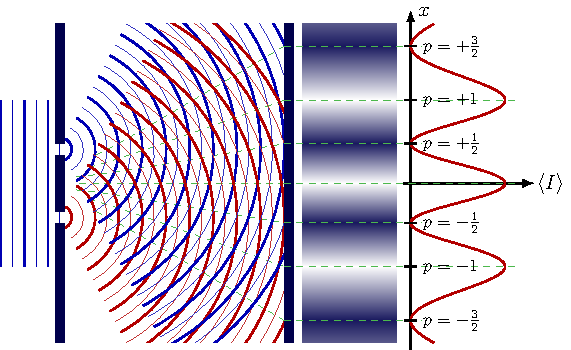
\includegraphics[width=\linewidth]{young_result}
	\end{center}
\end{minipage}

\begin{tcn}(obsv)<lftt>{Conclusion}
	Ainsi, il est clair que la lumière a un comportement ondulatoire. On peut donc
	songer que ce comportement est issu d'une collection d'objets individuels qui
	la composerait, des «~corpuscules~» de lumière~: les photons.
\end{tcn}

\section{Dualité onde-corpuscule}
\label{sec:dualondcorp}

\subsection{Définitions}
\label{ssec:docdef}
En physique classique (au \textsc{XIX}\ieme), le mouvement d'un corpuscule et
d'une onde sont très différents~:
\begin{tcb*}(defi){Onde et corpuscule}
	\begin{itemize}
		\item Un \textbf{corpuscule} est \textbf{localisé}, est soumis à des forces,
		      et obéit aux lois de \textsc{Newton}~;

		\item Une \textbf{onde} n'est \textbf{pas localisée} mais est
		      \textbf{étendue} dans l'espace, peut être diffractée et interférer.
	\end{itemize}
\end{tcb*}

\subsection{Nature corpusculaire de la lumière}
\label{ssec:lumcorp}
En 1900, Max \textsc{Planck}, pour expliquer le spectre des corps chauffés,
puis \textsc{Einstein}, en 1905, pour expliquer l'effet photoélectrique, font
émerger l'hypothèse que la lumière est composés de petits grains de lumières~:
les photons. Le plus petit paquets d'énergie échangé avec une radiation de
fréquence $\nu$ vaut $\Delta{E} = h\nu$ où $h$ est la constante de
\textsc{Planck}.

\subsubsection{Photons}
\label{sssec:photons}
\begin{tcb*}(defi){Photons}
	La lumière correspond au déplacement de particules appelées \textbf{photons}
	qui~:
	\begin{itemize}
		\item sont \textbf{sans masse}~: $m\ind{photon} = 0$~;
		\item se déplaçent à la célérité de la lumière ($c$ dans le vide, $c/n$
		      sinon)~;
		\item transportent \textbf{chacun} une énergie~:
		      \psw{%
			      \[
				      \Ec = h\nu = h \frac{c}{\lambda}
				      \qav
				      h = \SI{6.62606957e-34}{J.s}
			      \]
		      }%
		      \vspace{-15pt}
		\item ont comme quantité de mouvement
		      \[
			      \psw{%
				      \pf = \h \vv{k}
				      \qav
				      \h = \frac{h}{2\pi}
				      \qet
				      \norm{\vv{k}} = \frac{2\pi}{\lambda}
			      }%
		      \]
	\end{itemize}
\end{tcb*}

\begin{tcb}(appl){Énergie d'un photon}
	Calculer l'énergie transportée par un photo «~bleu~», puis un photon
	«~rouge~».
	\tcblower
	\begin{itemize}
		\item \psw{%
			      Pour $\lambda\ind{bleu} = \SI{400}{nm}$, $\xul{\Ec\ind{bleu} =
					      \SI{4.97e-19}{J}}$~;
		      }%
		\item \psw{%
			      Pour $\lambda\ind{rouge} = \SI{650}{nm}$, $\xul{\Ec\ind{rouge} =
					      \SI{3.06e-19}{J}}$.
		      }%
	\end{itemize}
\end{tcb}

\begin{tcb}(defi){Électron-volt}
	Plutôt que de parler en Joules, les unités étant petites, on exprime les
	énergies en \textbf{électron-volt}, correspondant à l'énergie cinétique gagnée
	par une particule de charge élémentaire lorsqu'elle est accélérée par une
	tension de \SI{1}{V}. On a alors
	\psw{%
		\[
			\SI{1}{eV} = \SI{1.602e-19}{J}
		\]
	}%
	\vspace{-15pt}
\end{tcb}

Pour l'application précédente, on trouve $\Ec\ind{bleu} = \SI{3.10}{eV}$
et $\Ec\ind{rouge} = \SI{1.91}{eV}$.

\subsubsection{Transitions atomiques}
\label{sssec:transatom}

\paragraph*{Introduction}
Pour expliquer l'effet photoélectrique, il faut encore justifier l'absorption
quantifiée. Pour cela, on établit (et ici on admet) le modèle suivant~:
\begin{tcb*}[sidebyside, righthand ratio=.35](prop){Transitions atomiques}
	L'énergie des électrons autour d'un atome ne peut prendre que certaines
	valeurs précises et est \textbf{quantifiée} en niveaux, entre le
	\textbf{fondamental} quand il est au repos et les niveaux \textbf{excités}
	sinon.
	\tcblower
	\begin{center}
		\sswitch{
			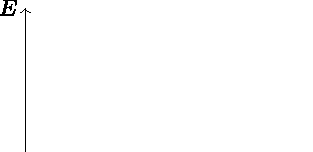
\includegraphics[width=\linewidth]{atome_niveau_stud}
		}{
			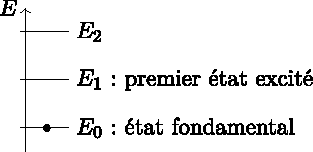
\includegraphics[width=\linewidth]{atome_niveau_prof}
		}
	\end{center}
\end{tcb*}

\paragraph*{Échanges d'énergie}
Il existe alors plusieurs modes d'échange d'énergie entre lumière et matière.
\smallbreak
\noindent
\begin{minipage}[t]{.70\linewidth}
	\begin{itemize}
		\item[b]{Absorption}: un photon d'énergie $h\nu$ arrive sur un atome dont un
		électron est sur le niveau d'énergie $\Ec$. Le photon peut alors être
		absorbé \textbf{seulement} s'il existe un autre niveau d'énergie $\Ec'$ tel
		que
		\psw{%
			\[
				\Delta{\Ec} = \Ec' - \Ec = h\nu
			\]
		}%
		auquel l'électron se retrouve alors.
		\bigbreak
	\end{itemize}
\end{minipage}
\hfill
\noindent
\begin{minipage}[t]{.25\linewidth}
	\vspace{0pt}
	\begin{center}
		\sswitch{
			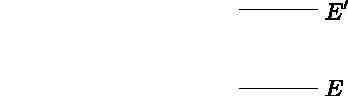
\includegraphics[width=\linewidth]{abs_stud}
		}{
			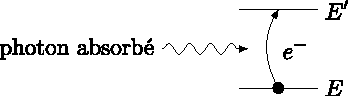
\includegraphics[width=\linewidth]{abs_prof}
		}
	\end{center}
\end{minipage}
Ainsi, \textbf{seules certaines longueurs d'ondes} peuvent être absorbées,
dépendant des composition atomiques.
\smallbreak
\noindent
\begin{minipage}[t]{.70\linewidth}
	\begin{itemize}
		\item[b]{Émission spontanée}: à l'inverse, un électron dans un état excité
		$\Ec'$ peut se \textbf{désexciter en émettant un photon}, en arrivant à
		l'état d'énergie $\Ec$. Le photon émis vérifie alors
		\psw{%
			\[
				\Delta{\Ec} = \Ec' - \Ec = h\nu
			\]
		}%
	\end{itemize}
\end{minipage}
\hfill
\noindent
\begin{minipage}[t]{.25\linewidth}
	\begin{center}
		\sswitch{
			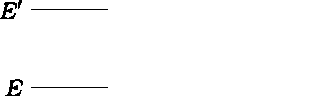
\includegraphics[width=\linewidth]{ems_stud}
		}{
			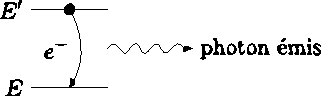
\includegraphics[width=\linewidth]{ems_prof}
		}
	\end{center}
\end{minipage}
\smallbreak
Ici aussi, il n'y a que \textbf{certaines longueurs d'ondes} pouvant être
émises.
\smallbreak
\begin{itemize}
	\item[b]{Émission stimulée}: dans certains cas, un électron à un niveau
	excité $\Ec'$ peut \textbf{recevoir un photon et en emmètre deux
		identiques}, en descendant l'électron à un niveau $\Ec$.
	\bigbreak
	C'est l'origine du LASER\ftn{\textit{Light Amplification by Stimulated
			Emission of Radiation}, ou «~amplification de la lumière par émission
		stimulée de radiation~» en français}.
\end{itemize}
\begin{center}
	\sswitch{
		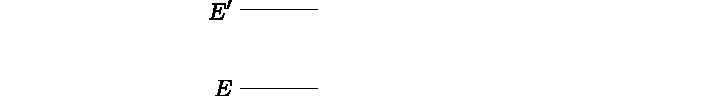
\includegraphics[width=.8\linewidth]{emsti_stud}
	}{
		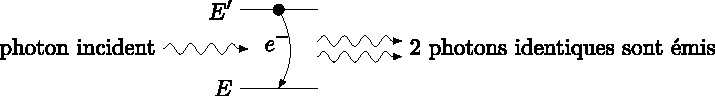
\includegraphics[width=.8\linewidth]{emsti_prof}
	}
\end{center}

\subsection{La matière~: onde et corpuscule.}
\label{ssec:matonde}
\subsubsection{Présentation}
\label{sssec:vidquantique}
Nous venons de voir que la lumière présentait un comportement à la fois
ondulatoire et à la fois corpusculaire. Cette dualité onde-corpuscule peut aussi
être étendue à la matière. Il est en effet possible d'observer avec des
électrons ou des petites molécules des franges d'interférences.
\begin{tcb}(exem)<lftt>"yout"{Vidéo}
	Une vidéo explicative de qualité est disponible à partir du site
	\url{https://toutestquantique.fr/dualite/}. Dans cette vidéo, les particules
	sont projetées sur une surface composée de deux fentes et on observe une figure
	d'interférences sur l'écran derrière. Si on bouche un des trous, la figure est
	radicalement différente, et signe de l'absence d'interférences.
	\smallbreak
	On observe alors que ces interférences n'émergent que si les particules
	«~passent par les deux trous~»~: ainsi, \textbf{la particule sur comporte
		comme une onde}.
\end{tcb}

En effet, si on a affaire à une particule matérielle, en laissant les deux
fentes ouvertes on devrait observer les deux séries d'impacts. Or, l'expérience
montre l'émergence d'impacts correspondants aux interférences~:
\begin{center}
	\sswitch{
		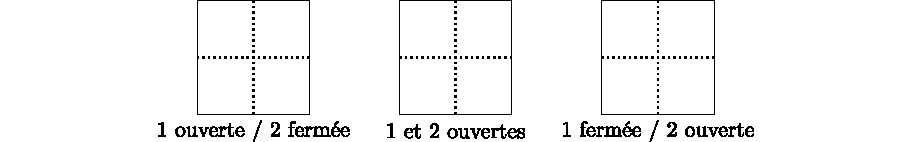
\includegraphics[width=\linewidth]{young_unique_stud}
	}{
		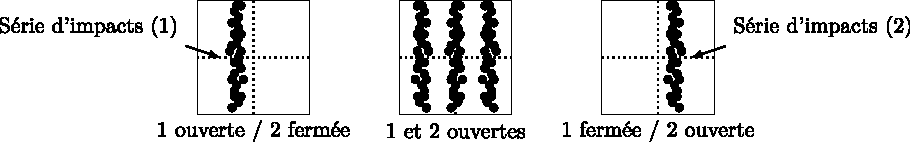
\includegraphics[width=\linewidth]{young_unique_prof}
	}
\end{center}
«~Pire~» encore, l'\textbf{observation perturbe la mesure} et semble «~annuler~»
les effets quantiques.

\subsubsection{Rappels de mécanique classique}
\label{sssec:rapmeca}
Avant d'entamer la suite, un rapide rappel de mécanique classique s'impose. Dans
toutes les théories établies jusque-là\ftn{\textbf{Attention}, en mécanique
	\textbf{non-relativiste} uniquement~: $v < \frac{1}{10}c$.}, le mouvement d'une
particule matérielle ($m \neq 0$ donc électrons, protons, balle de tennis…) est
décrit en particulier par~:
\begin{enumerate}
	\item Sa quantité de mouvement $\pf = m\vf$~;
	\item son énergie cinétique $\Ec_c = \frac{1}{2} mv^2$.
\end{enumerate}

\subsubsection{Longueur d'onde de \textsc{de Broglie}}
\label{sssec:lgdb}
Ainsi, pour quantifier les effets ondulatoires d'une particule de masse $m$ et
de vitesse $v$, on lui associe une longueur d'onde~:
\begin{tcb*}(defi){Longueur d'onde de \textsc{de Broglie}}
	Une onde de matière associée à une particule matérielle~:
	\begin{itemize}
		\item se propage à la vitesse $v$ de déplacement de la «~particule~»~;
		\item a pour longueur d'onde la longueur d'onde de \textsc{de Broglie}~:
		      \psw{%
			      \[
				      \boxed{\lambda\ind{DB} = \frac{h}{p}}
			      \]
		      }%
	\end{itemize}
	On a alors diffraction de matière possible si la fente est de
	largeur $a \lesssim \lambda\ind{DB}$.
\end{tcb*}

\begin{tcb}[breakable](appl)<lftt>{Longueur d'onde de matière}
	\begin{enumerate}
		\item Vérifier l'homogénéité de la formule précédente.
		      \smallbreak
		      \psw{%
		      $[h] = \si{J.s}$ soit $\si{kg.m^2.s^{-1}}$, d'où
		      \[
			      \left[\frac{h}{mv}\right] =
			      \frac{\si{kg.m^2.s^{-1}}}{\si{kg.m.s^{-1}}} = \si{s}
		      \]
		      }%
		\item Calculer la longueur d'onde de \textsc{de Broglie} d'une balle de
		      tennis d'une part, puis d'un électron allant à la vitesse $c/10$ d'autre
		      part. Les effets quantiques peuvent-ils se manifester à ces échelles~?
		      \smallbreak
		      \psw{%
			      \begin{itemize}
				      \item Pour une balle allant à $\SI{20}{m.s^{-1}}$ et pesant
				            \SI{50}{g}, on trouve
				            \[
					            \lambda\ind{DB,balle} = \SI{6e-34}{m}
				            \]
				            Il n'y a donc pas d'effet quantique à l'échelle de la balle.
				      \item Pour un électron de masse $m \approx \SI{e-30}{kg}$ à cette
				            vitesse, on trouve
				            \[
					            \lambda\ind{DB,é} = \SI{20}{pm}
				            \]
				            Ce qui est tout à fait dans l'ordre de grandeur de la taille d'un
				            atome.
			      \end{itemize}
		      }%
	\end{enumerate}
\end{tcb}

\section{Formalisme quantique}
\label{sec:formQ}
\subsection{Retour sur l'expérience}
\label{ssec:introprob}
Dans l'expérience des fentes d'\textsc{Young}, on peut se poser la question
suivante~: «~détecte-t-on la particule en un point M~?~». On introduit pour cela
la \textbf{probabilité de présence}~:
\begin{tcb*}(prop){Probabilité de présence}
	La probabilité de présence est une quantité mathématique, d'intégrale égale à 1
	sur son domaine de définition, telle qu'entre $x$ et $x+\dd{x}$ elle s'écrive
	\psw{%
		\[
			\dd{P} = p (x) \dd{x}
		\]
	}%
	avec $p (x)$ la \textit{densité de probabilité de présence} (ou «~probabilité
	ponctuelle~»)
\end{tcb*}
\noindent
\begin{minipage}[c]{.55\linewidth}
	\paragraph*{Si une fente est fermée}
	Si l'une des fentes est fermée, on observe une densité de probabilité de
	présence d'une forme pour le passage d'un obstacle~:
\end{minipage}
\hfill
\begin{minipage}[c]{.43\linewidth}
	\begin{center}
		\sswitch{
			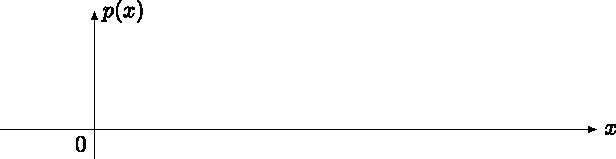
\includegraphics[width=\linewidth]{densprob_stud}
		}{
			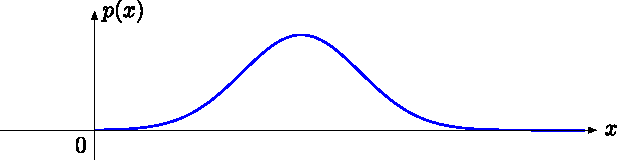
\includegraphics[width=\linewidth]{densprob_1fente_prof}
		}
	\end{center}
\end{minipage}
\begin{minipage}[c]{.55\linewidth}
	\paragraph*{Si les deux fentes sont ouvertes}
	Il se passe alors quelque chose de phénoménal pour une particule de matière~: la
	densité de probabilité de présence a l'allure suivante~:
\end{minipage}
\hfill
\begin{minipage}[c]{.43\linewidth}
	\begin{center}
		\sswitch{
			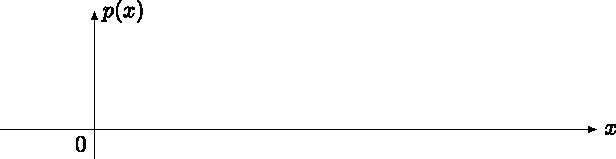
\includegraphics[width=\linewidth]{densprob_stud}
		}{
			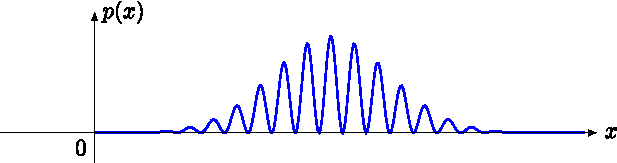
\includegraphics[width=\linewidth]{densprob_2fente_prof}
		}
	\end{center}
\end{minipage}

\begin{tcb*}(ror){Fentes d'\textsc{Young} et probabilité}
	Lors du passage d'une particule par deux fentes de faible largeur, \textbf{les
		densités de probabilités de présence ne se somment pas}~:
	\psw{%
		\[
			p (x) \neq p_1 (x) + p_2 (x)
		\]
	}%
	La densité totale semble donc émerger d'une grandeur plus fondamentale.
\end{tcb*}

\subsection{Notion de fonction d'onde}
\label{ssec:fonconde}
La grandeur qui s'additionne lorsque l'on superpose les situations 1 et 2 n'est
pas la densité de probabilité, mais la \textbf{fonction d'onde}\ftn{On retrouve
	la même notion avec les ondes «~classiques~»~: ce ne sont pas les amplitudes qui
	se somment, mais les signaux.}~:

\begin{tcb*}(defi){Fonction d'onde}
	On associe à une particule quantique une \textbf{fonction d'onde}, notée $\psi
		(\Mr,t)$ de \textbf{valeurs complexes} ($\psi \in \Cb$)~; on a alors
	\psw{%
		\[
			\boxed{p (\Mr,t) = \abs{\psi (\Mr,t)}^2}
			\qav
			P\ind{tot} = \int_{M \in \Vc} \abs{\psi(\Mr,t)}^2\dd{V}
			\Lra
			1 = \int_{-\infty}^{+\infty} \abs{\psi(\Mr,t)}^2 \dd{V}
		\]
	}%
	la probabilité de \textit{détecter} la particule au point $\Mr$ et à l'instant
	$t$.
\end{tcb*}

\begin{tcb*}[sidebyside](exem)<lftt>{Fonction d'onde et effondrement}
	\begin{center}
		\sswitch{
			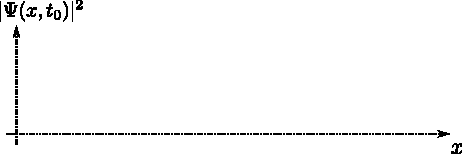
\includegraphics[width=\linewidth]{densprob_beforeafter_stud}
		}{
			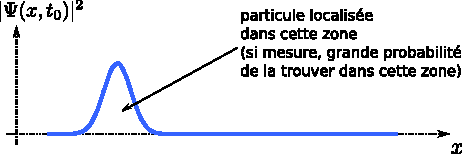
\includegraphics[width=\linewidth]{densprob_before_prof}
		}
		\captionof{figure}{Avant mesure.}
	\end{center}
	\tcblower
	\begin{center}
		\sswitch{
			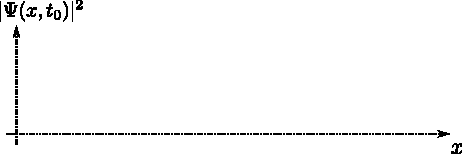
\includegraphics[width=\linewidth]{densprob_beforeafter_stud}
		}{
			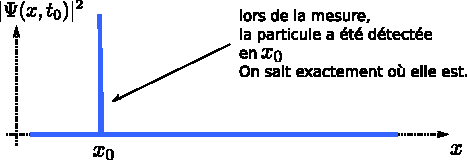
\includegraphics[width=\linewidth]{densprob_after_prof}
		}
		\captionof{figure}{Après mesure.}
	\end{center}
\end{tcb*}

\begin{tcb}(appl)<lftt>{Fonction d'onde pour les trous d'\textsc{Young}}
	Cette définition permet d'interpréter les trous d'\textsc{Young}. Soit
	$\psi(\Mr,t)$ la fonction d'onde résultant de la situation de superposition
	des deux fentes seules~:
	\begin{align*}
		\psi (\Mr,t) & =
		\psi_1(\Mr,t) + \psi_2(\Mr,t)
		\\\Ra
		p (\Mr)      & =
		\psw{\abs{\psi}^2 = \psi \psi^*}
		\\\Lra
		p (\Mr)      & =
		\psw{(\psi_1 + \psi_2)(\psi_1^* + \psi_2^*)}
		\\\Lra
		p (\Mr)      & =
		\psw{%
		\underbracket[1pt]{\psi_1\psi_1^*}_{p_1(\Mr)} +
		\underbracket[1pt]{\psi_2\psi_2^*}_{p_2(\Mr)} +
		\underbracket[1pt]{\psi_1\psi_2^* + \psi_1^*\psi_2}_{\text{interférences}}
		}%
	\end{align*}
\end{tcb}

\begin{tcb*}[breakable](impl){Conséquence de la fonction d'onde}
	Depuis l'introduction de cette notion, les débats sur l'interprétation de cet
	«~effondrement~» (ou plutôt «~réduction du paquet d'onde~») font rage entre
	les physicien-nes «~empiristes~»\ftn{\textsc{Bohr}, \textsc{Heisenberg},
		\textsc{Born}, \textsc{Dirac}…} (cf.\ interprétation de \textsc{Copenhague})
	et «~rationalistes~» (cf.\ interprétation des «~Mondes Multiples~»). Pour une
	approche vulgarisée, voir la vidéo de
	\href{https://www.youtube.com/watch?v=v3eSu9ac7Wk}{Science Étonnante -- Le
		plus gros problème de la mécanique quantique}.
	\bigbreak
	Quoiqu'il en soit, même loin de cette spécificité-là, la description de la
	matière par fonction d'onde rend \textbf{obsolète l'idée-même de trajectoire},
	puisqu'il devient impossible de connaître précisément la position d'une
	particule quantique.
\end{tcb*}

\subsection{Inégalité d'\textsc{Heisenberg}}
\label{ssec:heis}
Une autre implication majeure et intrinsèque de cette définition réside dans une
autre propriété de la mesure quantique~:
\begin{tcb*}[sidebyside, righthand ratio=.5, list entry={\lte Indétermina$^\circ$ quantique intrinsèque}](prop){Indétermination quantique intrinsèque}
	La mesure d'une grandeur $X$ sur un système quantique donne \textit{a priori}
	un résultat aléatoire, pris dans la distribution de la densité de probabilité
	$p(x)$, caractérisée par son écart quadratique $\Delta{X}$~:
	\psw{%
		\[
			\Delta{X} = \sqrt{\moy{X^2} - \moy{X}^2}
		\]
	}%
	\vspace{-15pt}
	\tcblower
	\begin{center}
		\sswitch{
			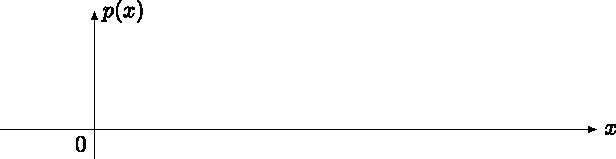
\includegraphics[width=\linewidth]{densprob_stud}
		}{
			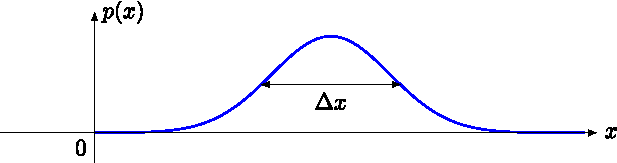
\includegraphics[width=\linewidth]{densprob_ecart_prof}
		}
	\end{center}
\end{tcb*}

\begin{tcb*}(impo){Écart-type vs.\ incertitude}
	Il est facile de plonger dans l'interprétation de cet écart comme une limite
	des instruments, mais ça serait passer à côté de toute la physique quantique.
	Tout aussi précis soit-il, un instrument mesurant de l'aléatoire plein de fois
	aura des valeurs aléatoires~!
\end{tcb*}

En mécanique quantique, la nécessité de prendre en compte le caractère
ondulatoire implique une indétermination sur la position et la quantité de
mouvement de la particule (une onde ne peut pas être parfaitement localisée), et
ce indépendamment de toute problématique de précision des mesures.

\begin{tcb*}(prop){Inégalité de \textsc{Heisenberg} spatiale}
	Soit une particule quantique repérée par sa position $x$ et par sa quantité de
	mouvement $p_x = mv_x$. Leurs écarts-types respectifs ne sont \textbf{pas
		indépendants}, et vérifient l'\textbf{inégalité de \textsc{Heisenberg}} (dite
	spatiale)~:
	\psw{%
		\[
			\Delta{x}\Delta{p_x} \geq \frac{\h}{2}
		\]
	}%
	La relation est presque vérifiée pour un système quantique.
\end{tcb*}

\begin{tcb}(rema)<lftt>"yout"{Vidéo}
	Pour un point de vue plus général sur cette inégalité et aller en profondeur
	sur son origine et \textit{les} inégalités de \textsc{Heisenberg}, je vous
	conseille infiniment vivement la vidéo de
	\href{https://youtu.be/MBnnXbOM5S4?si=trw2JoEydXDxsmM2}{3Blue1Brown -- The more
		general uncertainty principle, regarding Fourier transforms}
\end{tcb}

\section{Modèle semi-classique \textsc{Bohr}}
\label{sec:bohr}
\subsection{Principe}
\label{ssec:bohrprin}
On considère le mouvement d'un électron en orbite, au sens classique du terme,
autour d'un atome, mais on suppose que \textbf{son moment cinétique est
	quantifié}~:
\[
	\Lc_z = n \frac{h}{2\pi} = n\h
	\qav
	n \in \Nb
\]
\paragraph*{Hypothèses}
\begin{itemize}
	\item On néglige le mouvement du proton par rapport à celui de l'électron
	      ($\norm{\af_e}/\norm{\af_p} = m_p/m_e \approx \num{1800}$)~;
	\item On néglige la force gravitationnelle devant la force électrostatique
	      ($\norm{\Ff_g}/\norm{\Ff_e} = (4\pi \ep \Gc m_em_p)/(e^2) \approx
		      \num{e-40}$)~;
	\item on suppose le mouvement circulaire.
\end{itemize}

\subsection{Mise en équation}
\label{ssec:bohreq}
\noindent
\begin{minipage}[c]{.65\linewidth}
	On étudie le mouvement de l'électron, assimilé à un point matériel $\Mr$ dans le
	référentiel du proton, supposé galiléen. On utilise une base polaire $(\ur,\ut)$
	autour du proton.
	\bigbreak
	Le mouvement étant circulaire, on a~:
	\begin{align*}
		\vf & = \psw{r\tp \ut}
		\\
		\af & = \psw{-r\tp^2\ur + r \tpp \ut}
	\end{align*}
	La force subie par l'électron de la part du proton est~:
	\[
		\Ff_e = \psw{-\frac{1}{4\pi \ep_0}\frac{e^2}{r^2}\ur}
	\]
\end{minipage}
\hfill
\noindent
\begin{minipage}[c]{.33\linewidth}
	\begin{center}
		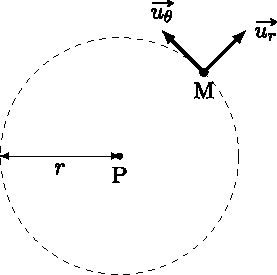
\includegraphics[width=\linewidth]{bohr_rota}
	\end{center}
\end{minipage}
D'après le PFD projeté sur la base polaire~:
\psw{%
	\[
		\left\{
		\begin{array}{rcl}
			-m_e r \tp^2 & = & - \frac{1}{4\pi\ep_0}\frac{e^2}{r^2}
			\\
			m_e r \tpp   & = & 0
		\end{array}
		\right.
		\qso
		\left\{
		\begin{array}{rcl}
			\tp & = & \sqrt{\frac{e^2}{4\pi\ep_0m_er^3}}
			\\
			\tp & = & \cte
		\end{array}
		\right.
	\]
}%
On détermine les orbites accessibles en utilisant l'hypothèse de
quantification, $\Lc_z = n\h$. Avec les données, on a
\psw{%
	\begin{gather*}
		\Lc_z = (\OM \wedge m_e \vf)\cdot \uz = m_ev_nr_n
		\Lra
		\Lc_z = \sqrt{\frac{m_ee^2r_n}{4\pi\ep_0}}
		\\\Ra
		\boxed{r_n = \frac{n^2\h^2 4\pi\ep_0}{m_e e^2}}
	\end{gather*}
}%
\noindent
\begin{minipage}[c]{.45\linewidth}
	L'énergie correspondante est alors
	\begin{DispWithArrows*}
		\Ec_m &= \Ec_c + \Ec_p
		\\
		&=
		\psw{\frac{1}{2}m_e r^2 \tp^2 - \frac{e^2}{4\pi\ep_0 r}}
		\Arrow{$\tp^2 = \frac{e^2}{4\pi\ep_0m_er^3}$}
		\\
		&=
		\psw{\frac{1}{2}m_er^2 \frac{e^2}{4\pi\ep_0m_er^3} - \frac{e^2}{4\pi\ep_0 r}}
		\Arrow{On simplifie}
		\\ &=
		\psw{- \frac{e^2}{8\pi\ep_0 r}}
		\Arrow{Pour $n \in \Nb$}
		\\\Lra
		\Aboxed{\Ec_{m,n} &= \psw{- \frac{m_e e^4}{8\ep_0^2 h^2}\frac{1}{n}}}
		\\
		\AN
		E_{m,n} &= - \frac{\SI{13.6}{eV}}{n^2}
	\end{DispWithArrows*}
\end{minipage}
\hfill
\begin{minipage}[c]{.45\linewidth}
	\begin{center}
		\sswitch{
			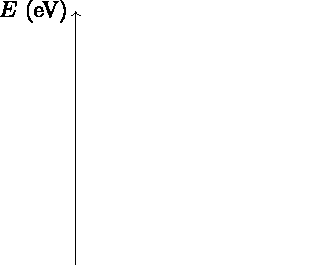
\includegraphics[scale=1]{bohr_spectra_stud}
		}{
			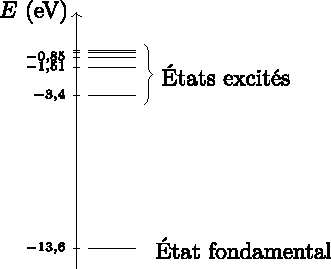
\includegraphics[scale=1]{bohr_spectra_prof}
		}
	\end{center}
\end{minipage}

\begin{tcb*}(ror){Modèle de \textsc{Bohr}}
	Même si cette approche a des défauts, elle a le mérite de \textbf{redonner le
		spectre d'absorption de l'hydrogène} entre deux couches $m$ et $n$, décrites
	par le physicien Johannes \textsc{Rydberg}~:
	\psw{%
		\[
			\frac{1}{\lambda_{n,m}} = R_H \left( \frac{1}{m^2} - \frac{1}{n^2} \right)
			\qav
			R_H = \frac{E_1}{hc} = \frac{m_e e^4}{8\ep_0^2 h^3 c} \approx \SI{1.10e7}{m^{-1}}
		\]
	}%
	Ainsi, une seule quantification permet rapidement de franchir un gap énorme
	de compréhension sur la structure du monde physico-chimique.
\end{tcb*}

\end{document}
